\section{基本工具}
\label{ch2}
\subsection{标题}
\label{ch2_1}
各级标题设计如下
\begin{lstlisting}[frame=single]
\section{}  %一级标题
\subsection{}  %二级标题
\subsubsection{}  %三级标题
\end{lstlisting}
模板规范了这些标题的格式,其他类型的标题比如
\begin{lstlisting}[frame=single]
\chapter{}
\end{lstlisting}
是不符合要求的。\par

\subsection{公式}
\label{ch2_2}
模板通过修改宏包设置规范公式格式,所以各种主要公式环境应该都是符合要求的比如
\begin{lstlisting}[frame=single]
\begin{equation}
\frac{x}{y}\times\sum_{i=1}^{\infty}\frac{1}{x^2}
\end{equation}
\end{lstlisting}
得到
\begin{equation}
\frac{x}{y}\times\sum_{i=1}^{\infty}\frac{1}{x^2}
\end{equation}
由于“工作手册”要求公式缩进两个字符左对齐,所以使用公式组的时候也应当左对齐。下面的情况影响美观
\begin{equation}
\begin{array}{rcl}
a\times c\times \alpha&=&b\\
d&=&e
\end{array}
\end{equation}
\par

\subsection{插图}
\label{ch2_3}
使用''figure''环境插图和命令
\begin{lstlisting}[frame=single,escapeinside='']
\caption{}
\end{lstlisting}
'插入标签是符合要求的,比如'
\begin{lstlisting}[frame=single]
\begin{figure}[H]
\centering
\subfigure['原始图像']{\label{figure:001} 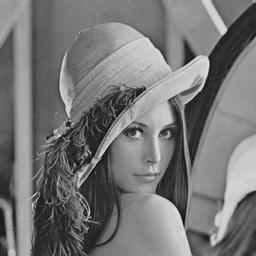
\includegraphics[width=0.4\textwidth]{001}}
\subfigure['噪声图像'($\mu=0,\sigma=20$)]{\label{figure:002} 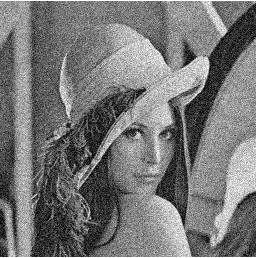
\includegraphics[width=0.4\textwidth]{002}}
\caption{'初始图像及噪声图像'}
\end{figure}
\end{lstlisting}
会得到
\begin{figure}[H]
\centering
\subfigure[原始图像]{\label{figure:001} 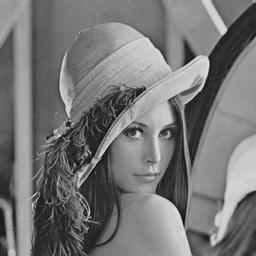
\includegraphics[width=0.4\textwidth]{001}}
\subfigure[噪声图像($\mu=0,\sigma=20$)]{\label{figure:002} 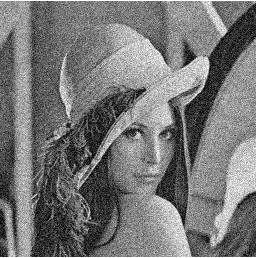
\includegraphics[width=0.4\textwidth]{002}}
\caption{初始图像及噪声图像}
\end{figure}
如果插图影响排版,多半是因为图片尺寸太大,或者一个环境中组合的图片数量太多。\par

\subsection{表格}
\label{ch2_4}

\subsection{脚注}
\label{ch2_5}